\documentclass[10pt]{IEEEtran}
\usepackage{preamble}


\begin{document}
\title{Mini-project 1: Tic Tac Toe}

\author{
   Federico Betti, Ivan Bioli\\
  \textit{CS-456 Artificial Neural Networks, EPFL Lausanne, Switzerland}
}


\maketitle

\begin{abstract}
In this report we present the results obtained from training an agent to play Tic-Tac-Toe both against quasi-optimal strategy (up to some user-defined degree of randomness) and by self-practice in an unsupervised fashion, then testing its performance against the optimal strategy and the fully random strategy. 
\end{abstract}

\section{Introduction}
\subsection{Notation}
We use throughout the report the same notation as in the project instructions, if not stated otherwise.

Moreover, in the following, we define as a \emph{win-booking state} every state in which the current player has the chance to win the game, either with the next move or in two moves with a fork, and similarly a \emph{block-win state} as every state in which the current player must block the chance of winning at the next turn of the adversary in order not to lose the game. Two examples of a \emph{win-booking state} and of a \emph{block-win state} are provided in \cref{plot_question_10}.

\section{Q-Learning}
Before discussing the results obtained with tabular Q-Learning, we clarify that in this section, in order to reduce the oscillations in the metrics that might occur during a particular training run, we averaged the results over 10 complete training runs. This helped us in particular to dump the oscillations which we observed for the measurements of $\mopt$, hence to obtain clearer plots of the training metrics. If not stated otherwise, throughout this section plots must be considered as averages over 10 training runs, with shaded regions possibly representing the standard deviation.

Furthermore, in most of the figures of the report, we then present only those values of the various parameters which we considered significant and representative the main trends, referring to the notebook attached to the submission for the complete results for all the tested values.

\subsection*{Question 1}
\Cref{plot_question1} shows an increase in average reward with experience, when training with $\epsilon = 0.1$ against \texttt{Opt(0.5)} for 20'000 games. At the end of training the average reward is positive, which indicates that the agent wins more games than it loses against \texttt{Opt(0.5)}. Hence the agent learns to play Tic-Tac-Toe.
%, even if in a sub-optimal way. Indeed \mopt\  and \mrand\  are lower than the ones obtained by the optimal policy.
% We choose here $\epsilon = 0.1$ as this enables us to carry out a fair comparison with the decaying exploration rule later on. Smaller values of $\epsilon$ were indeed performing better.
\begin{figure}[h]
    \centering
    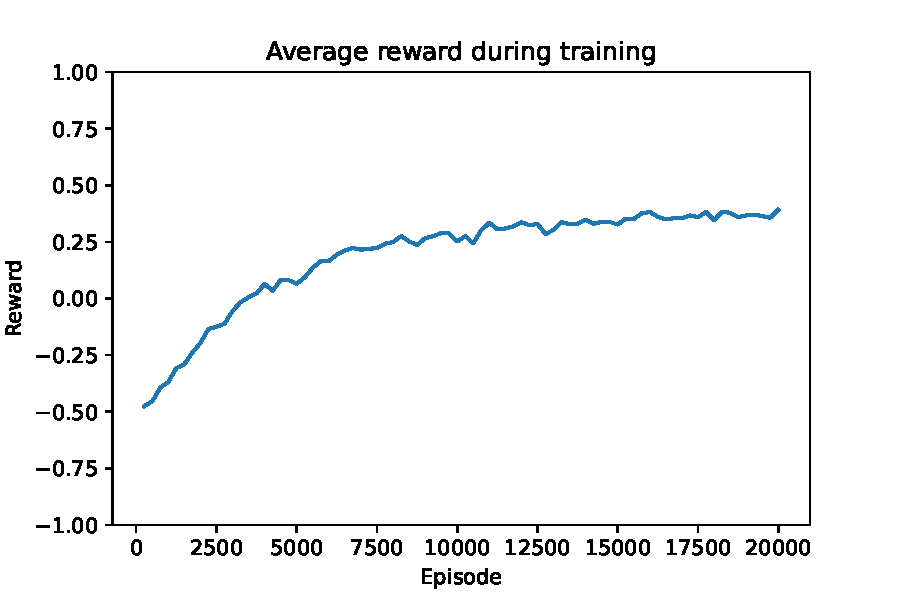
\includegraphics[width = 0.85\linewidth]{code/figures/rewards_Q1.pdf}
    \caption{Average reward for every 250 games during training with $\epsilon = 0.1$ against \texttt{Opt(0.5)} for 20'000 games.}
    \label{plot_question1}
\end{figure}

\subsection*{Question 2}
\Cref{plot_question2} shows the average reward during training for different values of $n^{*}$. In particular, we choose three values (including $n^{\star} = 1$, which corresponds to fixed exploration rate $\epsilon = \epsmin$) for which a good amount of the training episodes is played with constant $(1-\epsilon_{min})$-greedy policy, and a fourth value for which the exploration rate remains considerably high throughout the episodes. It can be observed that using $n^{\star} > 1$ in a first stage actions are chosen randomly more frequently and consequently the reward is lower than the one obtained with fixed $\epsilon = \epsmin$. However it can be observed that when $\epsilon(n)$ reaches $\epsmin$ the average reward approaches the same values seen for fixed exploration rate , but with the advantage of having explored more evenly the state space. On the other hand, for very large values of $n^{\star}$ we never reach the constant $(1-\epsmin)$-greedy policy, and therefore the average reward attains lower values as the agent keeps paying the price of exploration, never reaching the performance of the $(1-\epsmin)$-greedy agent. 

%% \Cref{secondplot_question2} analyses the reward trend for larger values of $n^{*}$, in particular values such that we never reach the constant $(1-\epsilon_{min})$-greedy policy. The average reward attains lower values as the agent keeps paying the price of exploration, never reaching the performance of the $(1-\epsilon_{min})$-greedy agent. For the same reason a stronger decay of $\epsilon$ achieves eventually the same reward as observed in \Cref{plot_question1}.

\begin{figure}[h]
    \centering
    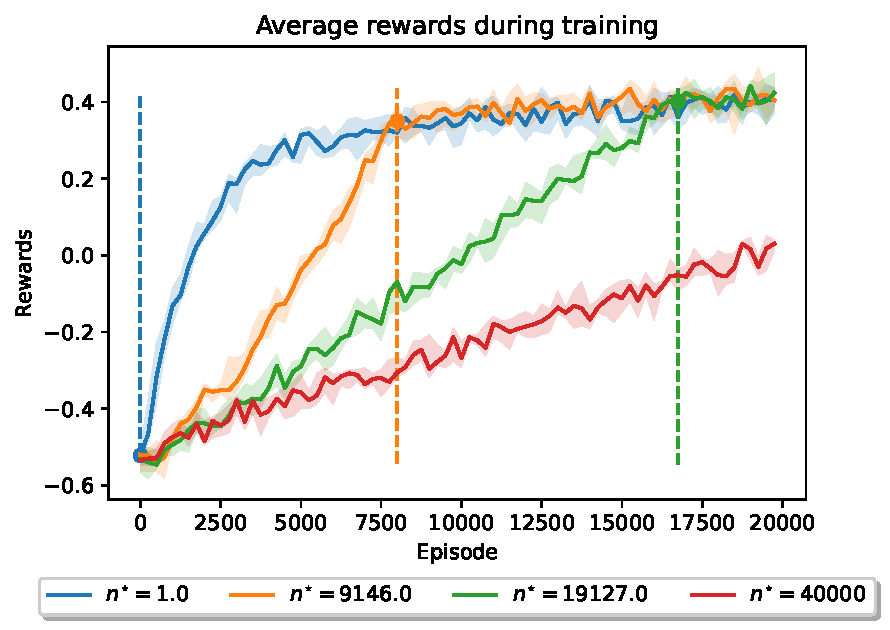
\includegraphics[width = 0.85\linewidth]{code/figures/rewards_n_star.pdf}
    \caption{Average rewards during training against Opt(0.5) for different values of $n^{*}$: the vertical lines correspond approximately to the episode at which the agent starts choosing moves with the minimum rate of exploration $\epsmin$ (for $n^{*} = 1$ this holds true from the very first episode).}
    \label{plot_question2}
\end{figure}

\subsection*{Question 3}
\Cref{plot_question3} shows the behaviour of \mopt\ and \mrand\ for different values of $n^{\star}$. Smaller values of $n^{*}$ are outperforming higher ones: indeed, in this second case the agent is not really able to play as exploration is prioritized throughout the whole learning process: hence \mopt\ remains relatively low and \mrand\ increases slowly as the agent is not taking advantage of the opponent's frequent wrong moves: this is coherent with the low rewards seen before. On the other hand, lower values of $n^{\star}$ are reaching asymptotically the same performance of the $(1-\epsmin)$-greedy agent, as observed for the rewards in \texttt{Question 2}.

\begin{figure}[h]
    \centering
    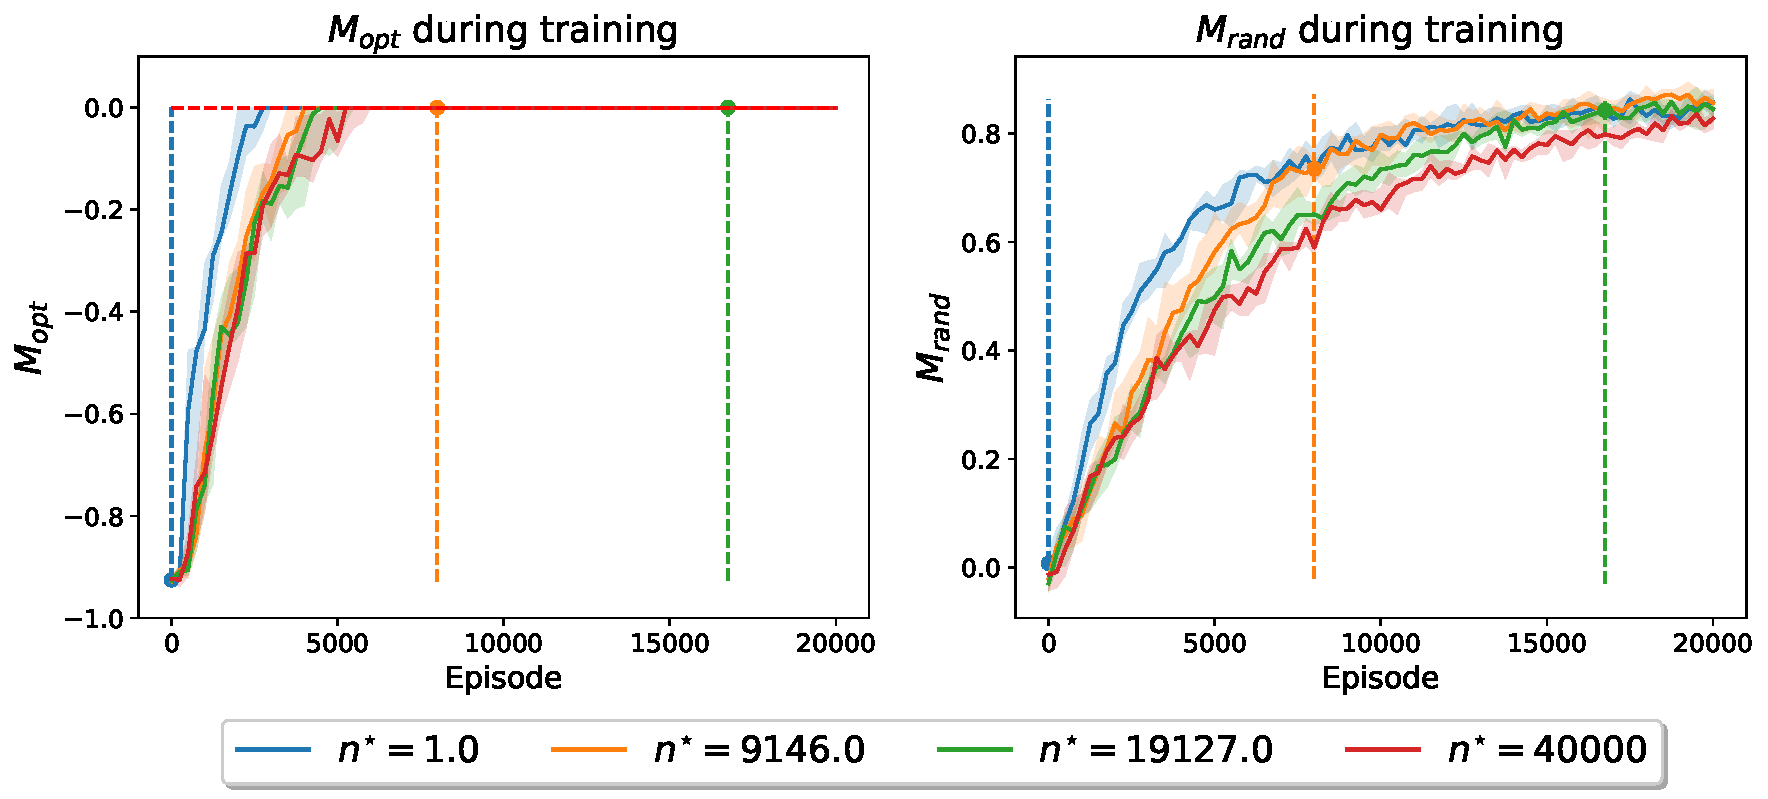
\includegraphics[width=\linewidth]{code/figures/performance_n_star.pdf}
    \caption{Behaviour of \mopt\  and \mrand\  every 250 training episodes for small values of $n^{*}$:  the vertical lines correspond approximately to the episode at which the agent starts choosing moves with the minimum rate of exploration $\epsmin$ (for $n^{*} = 1$ this holds true from the very first episode).}
    \label{plot_question3}
\end{figure}


\subsection*{Question 4}
\Cref{plot_question4} shows the performance measures \mopt\  and \mrand\  when training with Q-Learning against \texttt{Opt($\eopt$)} for different values of $\eopt$ and using decreasing exploration with $n^{*} = 19127$.

When training against \texttt{Opt(0)} the agent quickly learns to draw against the optimal player, and \mopt\  reaches 0. However, the performance against the random player \mrand\  does not improve significantly. This is because, when playing against the optimal player, there is no possibility of ending up in a \emph{win-booking state}. Hence, all the $Q$-values $Q(s_t, a)$ with $s_t$ a win-booking state are equal to their initialization value zero and when the agent plays against the random policy and possibly reaches a win-booking state, it chooses the next move randomly. 
Conversely, when training against \texttt{Opt(1)} \mrand\  quickly increases, while \mopt\  increases less sharply and without reaching zero. In this case, the agent learns to try to get a $+1$ reward taking advantage of possible mistakes of his opponent, even if this implies occasionally losing the game. 
Training against \texttt{Opt(0.5)} both \mopt\  and \mrand\  increase significantly. The agent is able to win against the random policy and to draw against the optimal one, but not as good as if trained against \texttt{Opt(0)} or \texttt{Opt(1)} respectively. The values $\eopt = 0.2$ and $\eopt = 0.8$ show intermediate results. 

In conclusion, the agent learns to gain optimal rewards (in expectation) against the opponent it is trained against. Indeed the optimal $Q$-values depend on the transition probabilities, which vary with the opponent. If compared with the agent trained against \texttt{Opt(0.5)}, choosing extreme values of $\eopt$ makes the agent gain little in one of the two performance measures and lose much in the other, resulting in a worse general performance.

\begin{figure}[h]
    \centering
    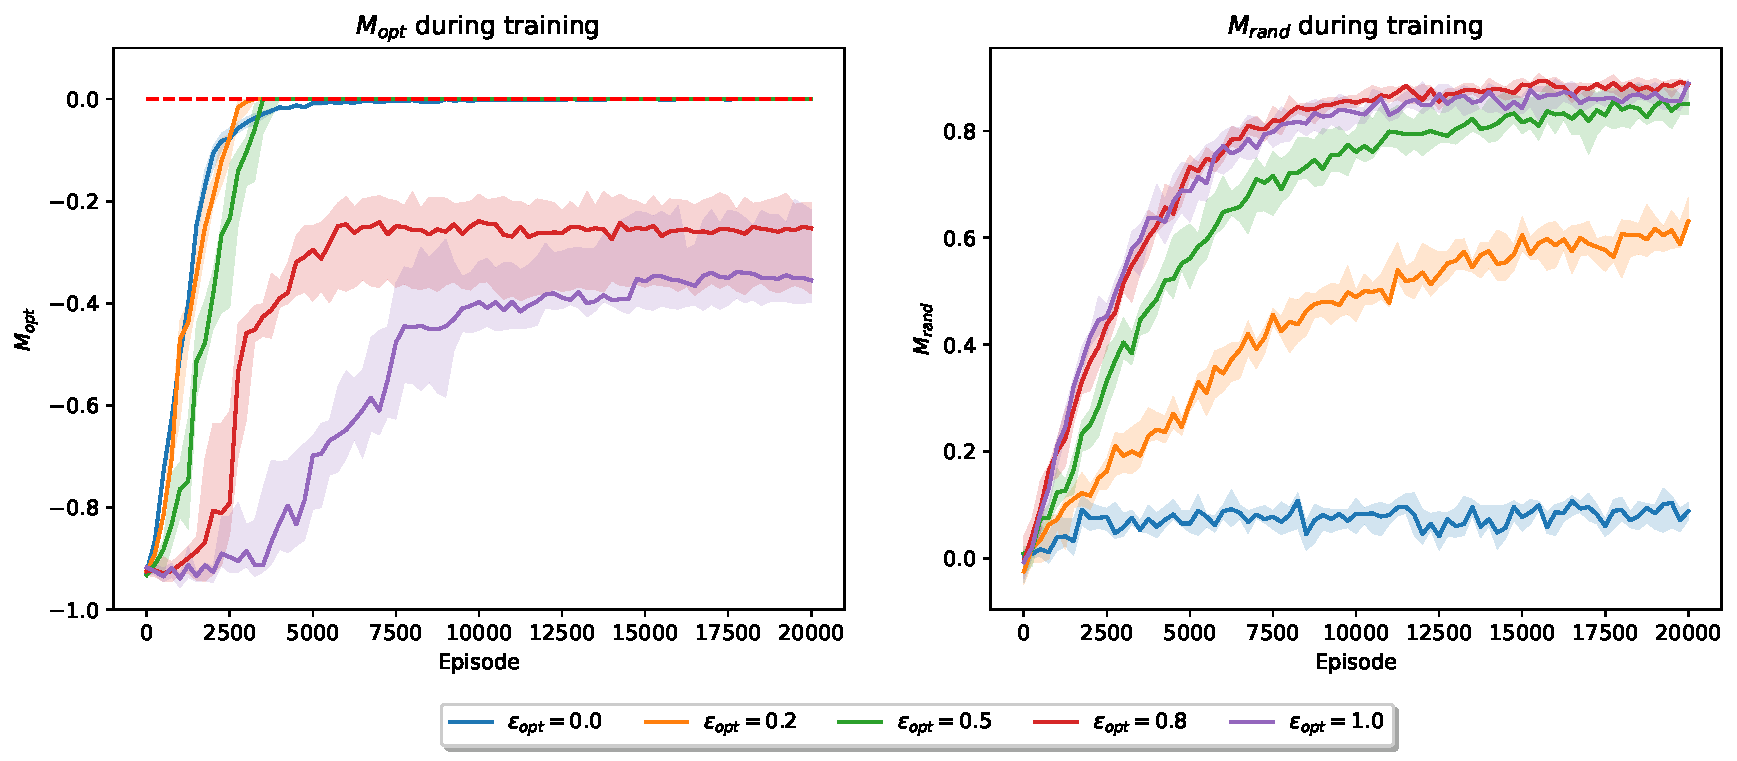
\includegraphics[width=\linewidth]{code/figures/performance_epsilon_opt.pdf}
    \caption{Behaviour of \mopt\  and \mrand\  every 250 training episodes for different values of \eopt.}
    \label{plot_question4}
\end{figure}

\subsection*{Question 5}
The highest values of \mopt\  and \mrand\  training with Q-Learning for $20000$ games against \texttt{Opt($\eopt$)} are achieved for \textcolor{red}{$\eopt = ...$} using decreasing exploration with $n^{\star} = 19127$, and they are equal to \textcolor{red}{$\mopt = ...., \, \mrand = ...$}.

\subsection*{Question 6}
We claim that $Q_1(s,a)$ and $Q_2(s,a)$ do not have the same values, as suggested by the experimental results shown in \emph{Question 4}.
Indeed, the optimal $Q$-values, i.e. those satisfying the Bellman equation, represent the total expected (discounted) reward and depend on transition probabilities, which are different if playing against \texttt{Opt(1)} or \texttt{Opt(0)}. 

Agent 1 during training never encounters win-booking states, hence at the end of the training $Q_1(s,a)$ is equal to the initialization value for every win-booking state $s$ and every action $a$. This is because the transition probability to any of this states is zero when playing against \texttt{Opt(0)}. Moreover, we expect $Q_1(s,a) = -1$ (possibly discounted by $\gamma$) for actions that make the opponent win (reward $-1$ at the end of the game) and $Q(s,a) = 0$ for all other actions, since Agent 1 can at most draw against \texttt{Opt(0)}. 

On the contrary, Agent 2 encounters win-booking states during training and we expect $Q_2(s,a) = 1$ (possibly discounted by $\gamma$) for actions that make the agent win, hence $Q_2(s,a) \neq Q_1(s,a)$. Furthermore we can expect $Q_2(s,a) \neq Q_1(s,a) = -1$ for actions that bring the opponent in a win-booking state, because the \texttt{Opt(1)} plays randomly and might not take the chance to win.

\subsection*{Question 7}
\Cref{plot_question7} shows the behaviour of \mopt\ and \mrand\ for different exploration rates $\epsilon$ of the learning agent. We observe that by training the agent with greedy policy its performance is poor both against \texttt{Opt(0)} and \texttt{Opt(1)} due to a poor exploration of the state space. It suffices to slightly increase $\epsilon$ (e.g. in expectation only a non-greedy action every 100) to improve majorly. On the other hand, a too large exploration rate causes poor performances for both \mopt\ and \mrand\ : indeed we expect that the empirical Q-values $Q(s_t, a)$, where $s_t$ is either a win-booking state or a block-win state, are not good estimates of the true ones.
%% unable to be deterministic in crucial moves and hence its behaviour against \texttt{Opt(0)} remains oscillatory, whereas its performance against \texttt{Opt(1)} is always tied or exceeded by smaller $\epsilon$ values.
\begin{figure}[h]
    \centering
    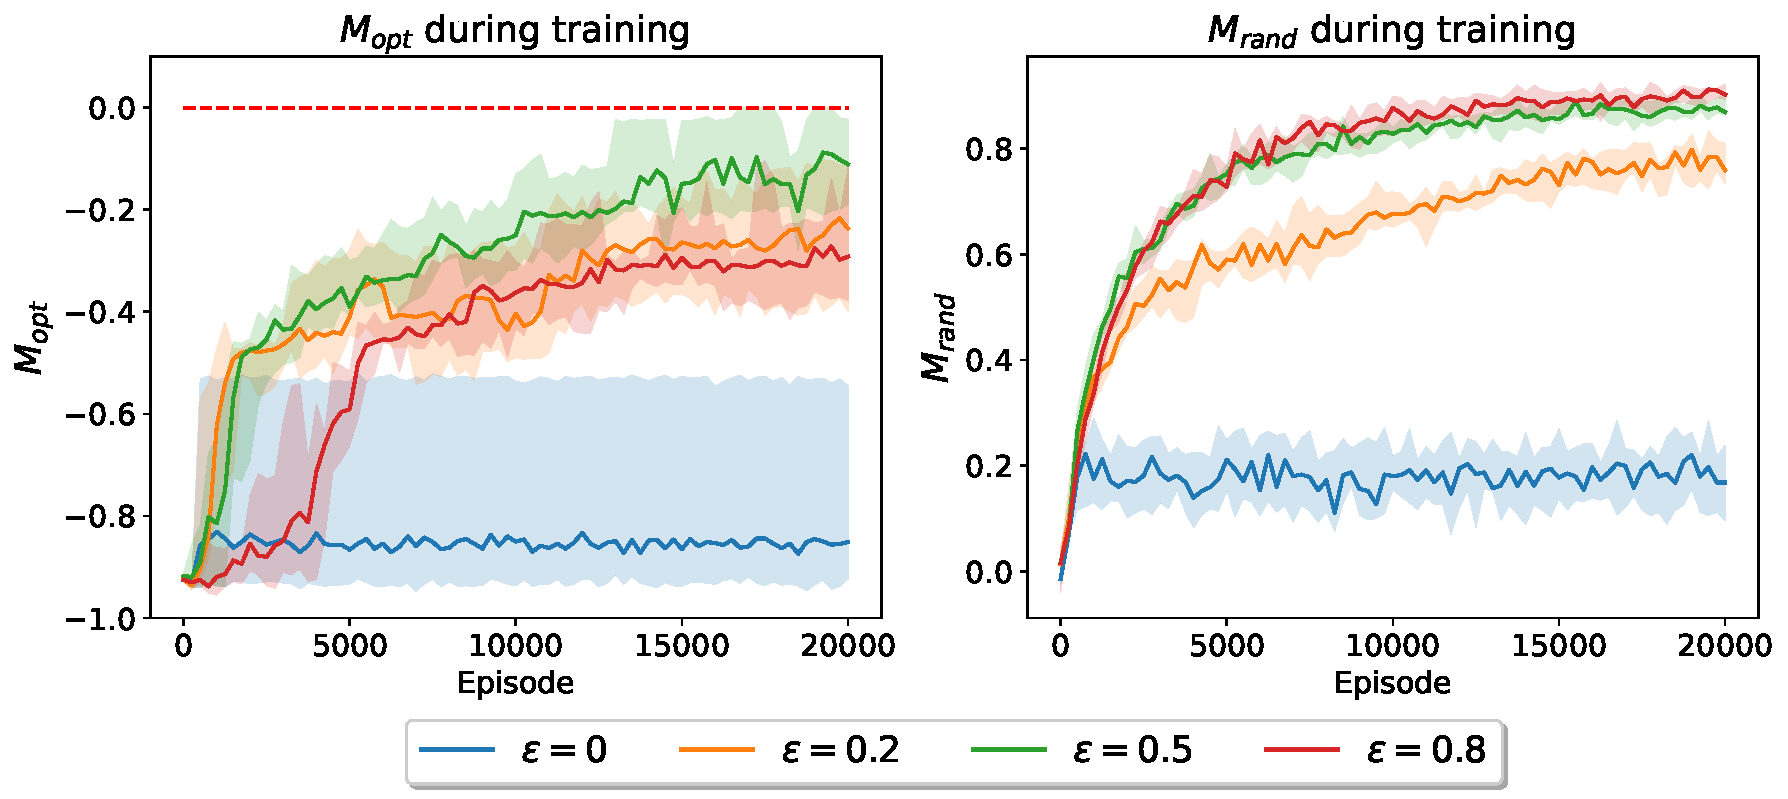
\includegraphics[width=\linewidth]{code/figures/performance_epsilon_self.pdf}
    \caption{Behaviour of \mopt\ and \mrand\ every 250 training episodes for different exploration rates $\epsilon$}
    \label{plot_question7}
\end{figure}


\subsection*{Question 8}
\Cref{plot_question8} shows the behaviour of \mopt\ and \mrand\ during training by self-learning, for different values of $n^{\star}$. We observe similar results to \emph{Question 3}: when we ensure with our choice of $n^{\star}$ that the agent plays a reasonable amount of the training episodes with minimum exploration rate the final performance is comparable to the one with fixed exploration rate, but with also the advantage of a wider exploration of the state space. With $n^{\star}$ too large, i.e. $n^{\star} = 40000$ in the plot, the agent keeps paying the price of exploration and does not reach the performance of $n^{\star} = 1$, especially in terms of \mopt.

\begin{figure}[h]
    \centering
    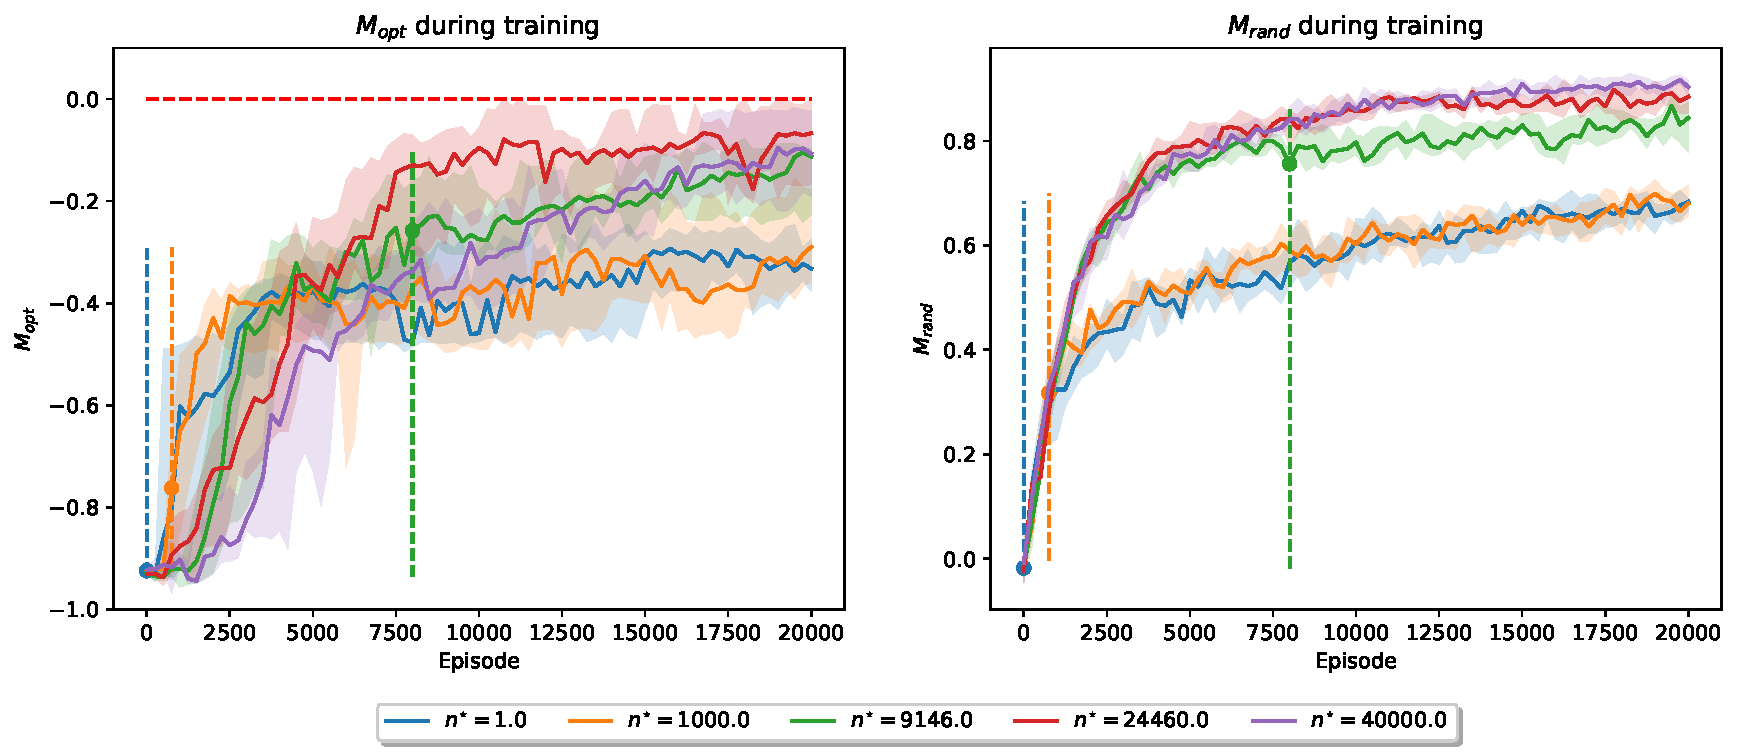
\includegraphics[width=\linewidth]{code/figures/performance_n_star_self.pdf}
    \caption{Behaviour of \mopt\ and \mrand\ over the training episodes for different values of $n^{\star}$:  the vertical lines correspond approximately to the episode at which the agent starts choosing moves with the minimum rate of exploration $\epsmin$.}
    \label{plot_question8}
\end{figure}



\subsection*{Question 9}
The highest values of \mopt\  and \mrand\  training with Q-Learning by self practice for $20000$ games are achieved using decreasing exploration with $n^{\star} = 19127$, and they are equal to \textcolor{red}{$\mopt = ...., \, \mrand = ...$}.

\subsection*{Question 10}
%\Cref{plot_question_10} shows the $Q$-values of available actions for three significant board arrangements in which player X has the chance to win, to block a win of player O or to win for sure in two or more moves.
In \Cref{fig_heatmap_1} the highest $Q$-value correctly corresponds to the action that makes the agent (player X) win, and it is equal to 1, i.e. the reward. However, playing in any of the other empty corners would also lead to winning the game in two moves. Similarly, in \Cref{fig_heatmap_3} the agent correctly picks the center, which brings to victory in at most two moves and indeed has a $Q$-value close to $\gamma^2 = 0.98$, but other win-leading moves such as the south-east corner have a Q-value significantly lower than one. In \Cref{fig_heatmap_2} the agent (player O) correctly blocks the win of the adversary, predicting a negative reward for any other action.

It can be argued that the agent learned the game quite well. In the explored scenarios most of the Q-values do make sense and the agent plays one of the possible correct actions. However, the number of possible state-action pairs is too high to be sufficiently explored in $20000$ training episodes, hence not all of the $Q$-values converged to their optimal value. 

\begin{figure}[h]
     \centering
     \begin{subfigure}[t]{0.32\linewidth}
         \centering
         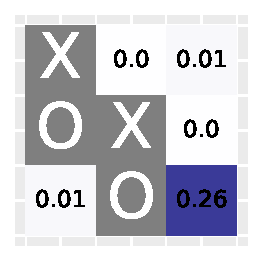
\includegraphics[width=\linewidth]{code/figures/heatmap_0.pdf}
         \caption{Chance of win}
         \label{fig_heatmap_1}
     \end{subfigure}
     \hfill
     \begin{subfigure}[t]{0.32\linewidth}
         \centering
         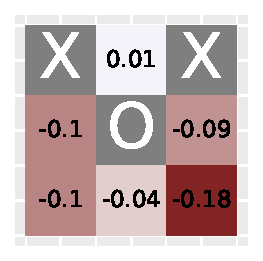
\includegraphics[width=\linewidth]{code/figures/heatmap_1.pdf}
         \caption{Chance of block}
         \label{fig_heatmap_2}
     \end{subfigure}
     \hfill
     \begin{subfigure}[t]{0.32\linewidth}
         \centering
         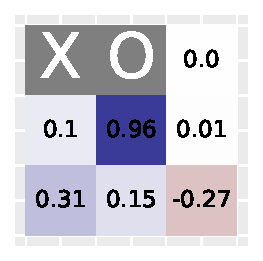
\includegraphics[width=\linewidth]{code/figures/heatmap_2.pdf}
         \caption{Chance to win or fork in the next move.}
         \label{fig_heatmap_3}
     \end{subfigure}
        \caption{$Q$-values of available actions in three different board arrangements, where player who makes the first move is always X.}
        \label{plot_question_10}
\end{figure}

\section{Deep Q-Learning}
\subsection*{Question 11}
\subsection*{Question 12}
\subsection*{Question 13}
\subsection*{Question 14}
\subsection*{Question 15}
\subsection*{Question 16}
\subsection*{Question 17}
\subsection*{Question 18}
\subsection*{Question 19}
\subsection*{Question 20}
\subsection*{Question 21}

\section*{Questions to be asked}
\begin{enumerate}
    \item La caption delle figure conta nel conteggio delle parole? Bisogna presentare la risposta alle domande tutta nella caption del plot?
    \item Inizializzazione dei Q-values per la domanda 6 
\end{enumerate}


\nocite{*}
\printbibliography

\clearpage
\detailtexcount{main}

\end{document}